\begin{table}
  \centering
  \caption{Evaluation per day of year}
  \label{tab:eval_doy}
  \begin{tabular}{rrrr}
  \(date\) & \(n\) & \(MAE\) & \(\sigma\) \\
  \hline 
  01.03.   &  103  &   26.14 &  36.35 \\
  02.03.   &  185  &   23.64 &  29.54 \\
  03.03.   &  286  &   21.24 &  24.80 \\
  04.03.   &  521  &   39.06 &  36.61 \\
  05.03.   & 1091  &   67.32 &  47.67 \\
  06.03.   & 1082  &   51.28 &  45.73 \\
  07.03.   &  925  &  204.89 & 127.97 \\
  08.03.   &  969  &  186.90 & 172.56 \\
  09.03.   & 1050  &   20.70 &  28.86 \\
  10.03.   & 1085  &   25.24 &  27.12 \\
  11.03.   &  586  &   30.31 &  40.46 \\
  \end{tabular}
\end{table}


The functionality of the system will be verified by doing regular predictions and comparing these to the actual 
parking situation later. Similar to the crawling implementation, the web application will generate a new prediction 
``15 minutes into the future''. These predictions will be saved in a database. 

To measure the error, we will use the mean absolute error 
\[
MAE \defeq mean(|y_i^∗ - y_i|)\text{,}
\]
where \(y_i^∗\) denotes the predicted value and \(y_i\) denotes the actual, crawled value. Table \ref{tab:eval_doy} lists the evaluation results fetched on 11.03.2017 around 6pm. 

The evaluations show that the predictions got worse on the 4th and are especially bad on the 7th and 8th March. The cause for this was some experimentation with the training method and the model.

On the 4th, the training method was adapted. Instead of generating 10 GradientBoostTrees with shrinkage values from 
\(0.1\) to \(1\) (step width \(0.1\)), only 4 GradientBoostTrees with fixed shrinkage values of (\(0.001\), \(0.01\), 
\(0.1\), and \(1\) were generated. According to \href{http://haifengl.github.io/smile/index.html#gbm}{the documentation of GradientBoost}, 
the shrinkage parameter controls the learning rate; it was assumed that picking a set of four very different values
would sufficient for good predictions.

On the 7th, the model attributes ``week of month'' and ``week of year'' were removed. All Learning models compute the 
so-called importances of the attributes used for learning. According to the importances determined in previous 
predictions, the aforementioned attributes were not important. Also, from this day on the attributes were normalized 
when training the model. This was not necessary but I wanted to try it out anyway.

As one can see in Table \ref{tab:eval_doy} both changes did not improve the model but instead made predictions worse. Therefore the changes were rolled back on the 9th. After this was done, the prediction accuracy increased again. 
Figures \ref{fig:actual} and \ref{fig:predictions} display the actual availability respectively the predicted 
availability of parking spaces over the last 48 hours. As one can see, the tendency of the predictions is quite good. However, the predictions tend to overshoot and ``wiggle around''. When presenting the intermediate results in class, it was suggested to dampen the predictions. 

\begin{figure}
  \centering
  \caption{Crawled parking space availability}
  \label{fig:actual}
  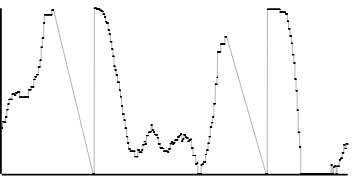
\includegraphics[scale=0.5]{fig_actual}
\end{figure}

\begin{figure}
  \centering
  \caption{Predicted parking space availability}
  \label{fig:predictions}
  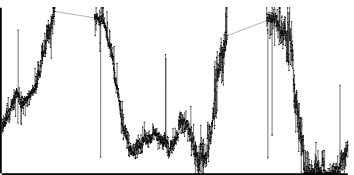
\includegraphics[scale=0.5]{fig_predictions}
\end{figure}
